\documentclass[a4j]{jsarticle}
\usepackage[dvipdfmx]{graphicx}
\usepackage{amsmath}
\usepackage{url}

\title{DBSCANの概要}
\author{大阪大学 工学部 電子情報学科 3年\\情報システム工学コース\\08D23091\,辻\,孝弥}
\date{\today}

\begin{document}
\maketitle

\section{DBSCANとは}

Density-Based Spatial Clustering of Applications with Noise(DBSCAN)は,データ分布の\textbf{密度}に着目してクラスタを抽出する手法である.1996年にMartin~Esterらが提案して以来,密度が高い領域をクラスタとしてまとめ,低密度領域の点をノイズ(外れ値)として切り捨てるシンプルさと汎用性から,機械学習分野で広く採用されている.

DBSCANの特徴は,\emph{クラスタ数を事前に与える必要がない}点にある.データ空間内で互いに近い点が多数存在する高密度領域を自動で検出し,それぞれをクラスタとみなす.周囲に点がほとんど存在しない孤立点はノイズとして扱われるため,異常検知にも応用できる.

\section{検索トレンドの動向}
図\ref{fig:trends}はGoogle~Trendsによる「DBSCAN」と「k\,\-means」の検索数推移を示す.近年,AI・データサイエンスへの関心が高まったことでDBSCANの検索数も増加傾向にある.k\,\-meansは古くから用いられてきたが,クラスタ数の事前指定が不要という利点からDBSCANも同程度に検索されるようになってきたと考えられる.

\begin{figure}[htbp]
  \centering
  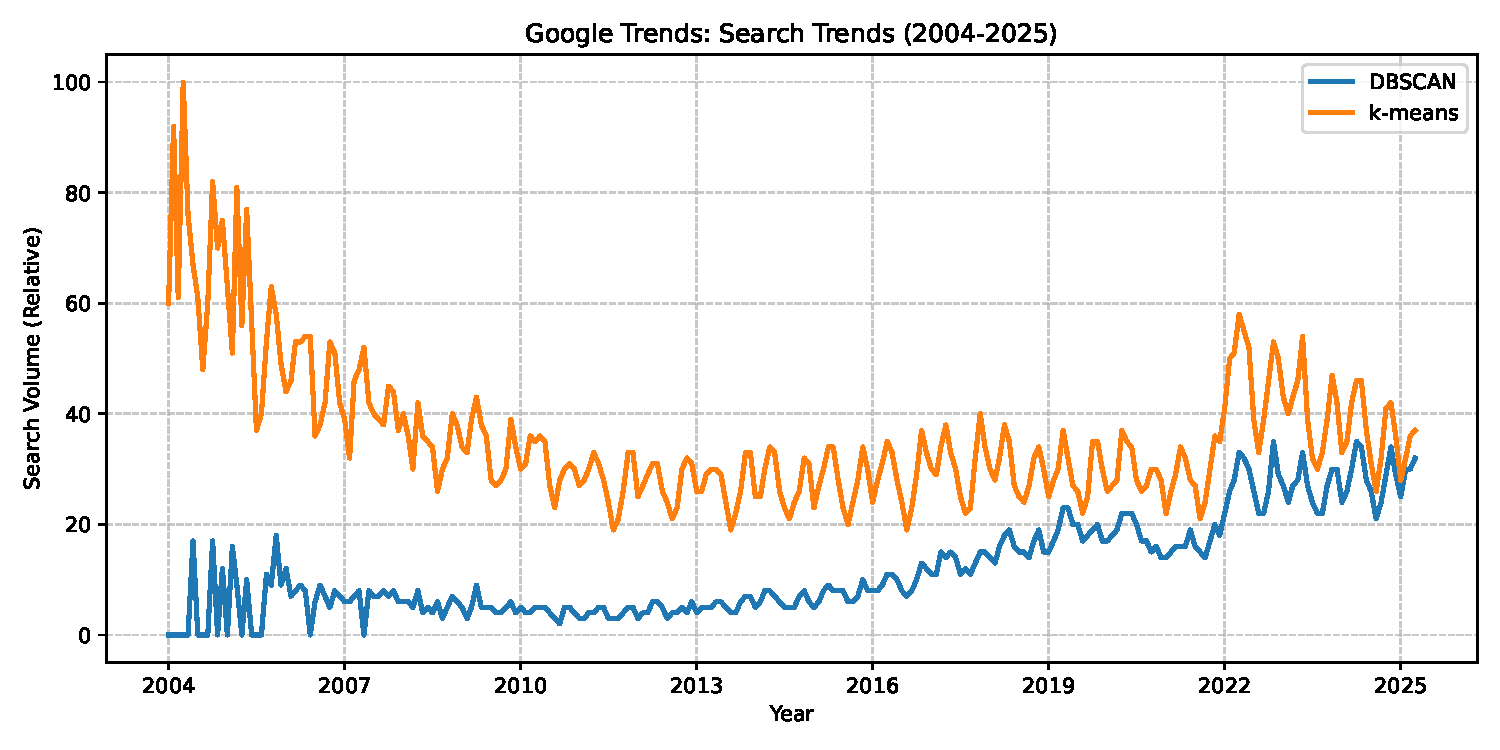
\includegraphics[width=0.7\textwidth]{trends_comparison.pdf}
  \caption{k\,\-means と DBSCAN の検索数比較}
  \label{fig:trends}
\end{figure}

\section{アルゴリズムの要点}

\subsection{2つの主要パラメータ}

DBSCANは,半径$\varepsilon$の近傍と最小点数$\text{MinPts}$という2つのパラメータで動作する.

\begin{description}
  \item[$\varepsilon$:] 半径$\varepsilon$以内に存在する点集合をその点の$\varepsilon$‐近傍と定義する.
        \[
          N_{\varepsilon}(p)=\{\,q \mid \mathrm{dist}(p,q)\le \varepsilon\,\}
        \]
  \item[MinPts:] 近傍に含まれる点数がMinPts以上なら,点$p$を\textbf{コア点}と呼ぶ.
\end{description}

\begin{itemize}
  \item \textbf{コア点}: $\varepsilon$‐近傍にMinPts以上の点を持つ点.
  \item \textbf{境界点}: 自身はコア点でないが,あるコア点の$\varepsilon$‐近傍に含まれる点.
  \item \textbf{ノイズ点}: いずれのコア点からも到達できない点.
\end{itemize}

\subsection{処理手順}
\begin{enumerate}
  \item すべての点を未訪問とする.
  \item 未訪問点$p$を1つ取り出し,$N_{\varepsilon}(p)$を求める.
  \item $|N_{\varepsilon}(p)|\ge\text{MinPts}$であれば新しいクラスタを生成し,$p$および$N_{\varepsilon}(p)$をクラスタに割り当てる.
  \item クラスタに追加された各点$q$について,再帰的に$N_{\varepsilon}(q)$を調べ,条件を満たす点をクラスタへ拡張する.
  \item $|N_{\varepsilon}(p)|<\text{MinPts}$の場合,$p$を一旦ノイズとラベル付けする.
  \item 未訪問点がなくなるまで手順2–5を繰り返す.
\end{enumerate}

\subsection{パラメータ選択の指針}

$\varepsilon$が小さすぎるとノイズが増え,大きすぎると異なるクラスタを誤って結合する.適切な値はデータに依存するため,\emph{k\,\-距離プロット}でエルボー点を探す方法がよく用いられる.MinPtsは次元数$D$に対して$D+1$以上を目安とするのが経験則である.

\clearpage
\section{k\,\-means との比較}

k\,\-meansはクラスタを凸形状(球状)と仮定し,クラスタ数を事前に指定する必要がある.非凸形状や異なる密度のクラスタが混在する場合,k\,\-means は適切に分割できないことが多い.これに対しDBSCANは形状の仮定を置かず,密度の差を利用して図\ref{fig:dbscan}のような複雑なクラスタも検出できる.

\begin{figure}[htbp]
  \centering
  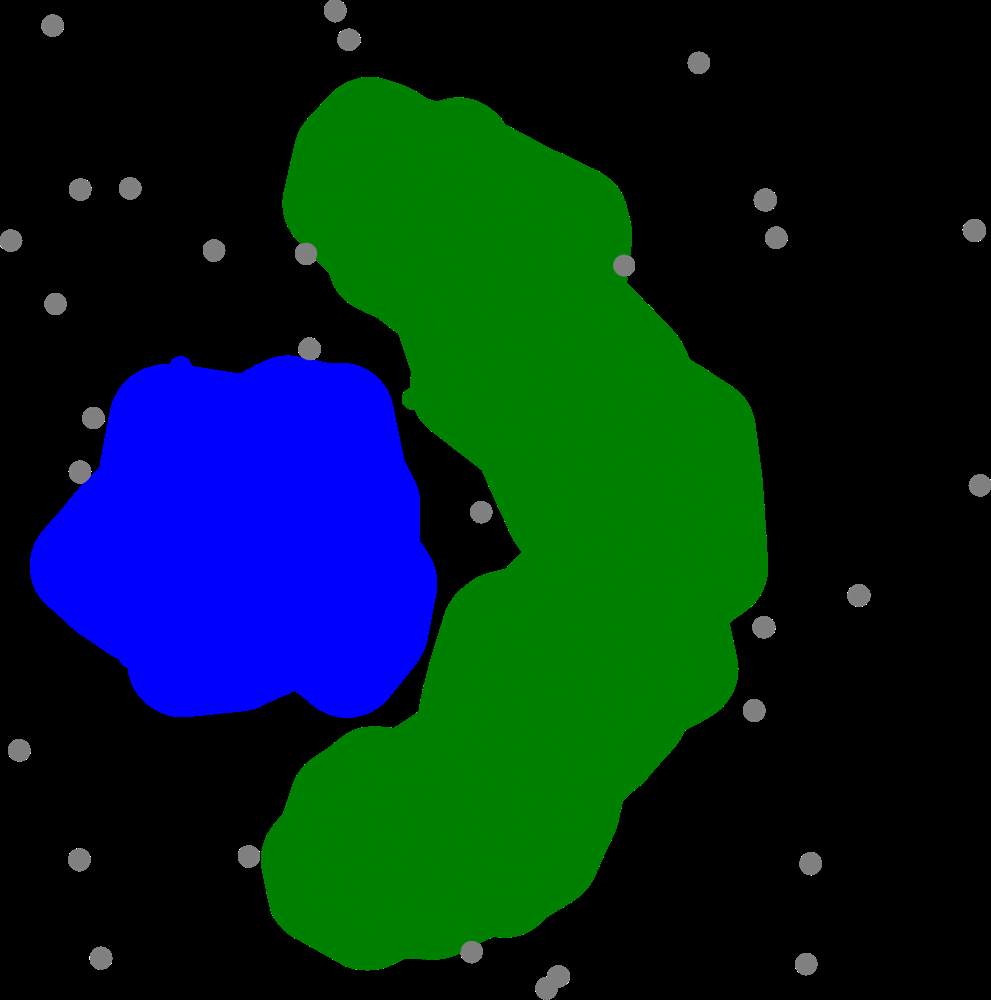
\includegraphics[width=0.3\textwidth]{31d42bec-0995-4e7d-9d96-cb806a43999e.png}
  \caption{DBSCAN による非凸クラスタの抽出例}
  \label{fig:dbscan}
\end{figure}

\section{おわりに}

DBSCANは,クラスタ数の事前設定が不要であり,任意形状のクラスタを検出できるという強みを持つ.適切なパラメータ設定が難点ではあるが,k\,\-距離プロットなどを活用することで実用上の課題は緩和できる.今後も異常検知や空間データ解析といった分野で重要な役割を果たすだろう.

\begin{thebibliography}{99}
  \bibitem{geeksforgeeks} DBSCAN Clustering in ML | Density based clustering,\
        \url{https://www.geeksforgeeks.org/dbscan-clustering-in-ml-density-based-clustering/},\\
        (最終アクセス: 2025‑01‑29).
  \bibitem{wikipedia} Wikipedia, ``DBSCAN,''\\
        \url{https://ja.wikipedia.org/wiki/DBSCAN},\\
        (最終アクセス: 2017‑04‑26).
\end{thebibliography}

\end{document}
